\chapter{Related Work}
\label{ch:related}

Many researchers have contributed to the WSN field, all focusing on different areas.
There are a few different aspects of WSNs that are considered in this thesis. To reflect this, the 
related work is grouped by different areas of WSN research. 

Areas
of WSN research include radio transceiver technology which has been 
developed for decades, but has only recently been developed as a low-power
technology. WSN research also includes MAC layer protocols, which are used by radios to share 
a radio channel between multiple devices. 
To move messages towards the sink, WSN nodes can either create 
clusters (Clustering Protocols), or communicate without clusters (Non-clustering Protocols).
There are benefits to using clusters in WSNs, and other benefits to not using clusters. 
Finally, heterogeneity in WSNs can be used
to improve the performance of a WSN.


\section{Wireless Sensor Networks}

% http://en.wikipedia.org/wiki/History_of_radio
Wireless technologies are by no means a new invention. In 1892
Nikola Tesla proposed that radio waves could be used for communication
without any wires connecting the two points~\cite{telsa}.
Since then, wireless radios have evolved from large, power 
hungry devices such as radio backpacks used in World War II, to 
%http://www.ww2gyrene.org/equipment_SCR_300.htm
%\begin{figure}[htbp]
%    \centering
%        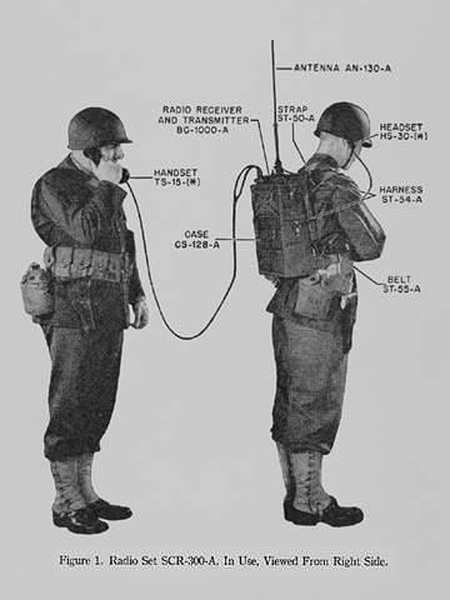
\includegraphics[height=3in]{images/relatedWork/Scr300.png}
%    \caption{A backpack radio as used in World War II. (Image via PD-USGOV)}
%    %http://en.wikipedia.org/wiki/File:Scr300.png
%    \label{fig:images_relatedWork_Scr300}
%\end{figure}
the ubiquitous cell phone of today. Wireless radios have gotten smaller,
more power efficient and much more affordable. 

The story of the computer has much in common with the evolution of the 
wireless radio. Starting with computers that were large and extremely expensive, 
computers are now standard equipment for everyday use. The
cost of computers has gone way down, as has the size of computers. Both wireless
radios and computer are core components of WSN nodes.

The paper that is often credited in being the first paper on designing WSNs is 
Pottie and Kaiser's~\cite{WINSProject}  \emph{Wireless Integrated Network Sensors}.
Pottie and Kaiser proposed the acronym WINS for the field, and were the first
to connect the ideas of pervasive low power computing with sensor networks and proposed an
architecture to help solve these problems. 
At its core WSNs are just microcontrollers, sensors and 
wireless radios; Pottie and Kaiser saw the potential of these
objects, and showed the world that the combination is more than the sum of its parts. 
The authors moved beyond looking at the components, and considered what could be possible
with the concept, and how it would need to be achieved. Pottie and Kaiser 
saw that the density of the distributed network is the strength of WSNs. Key points of the 
paper were that using the shortest transmission range is important
to increase node lifespan, and that networks must be self-organizing to work efficiently.

\begin{figure}[tb]
	\centering
		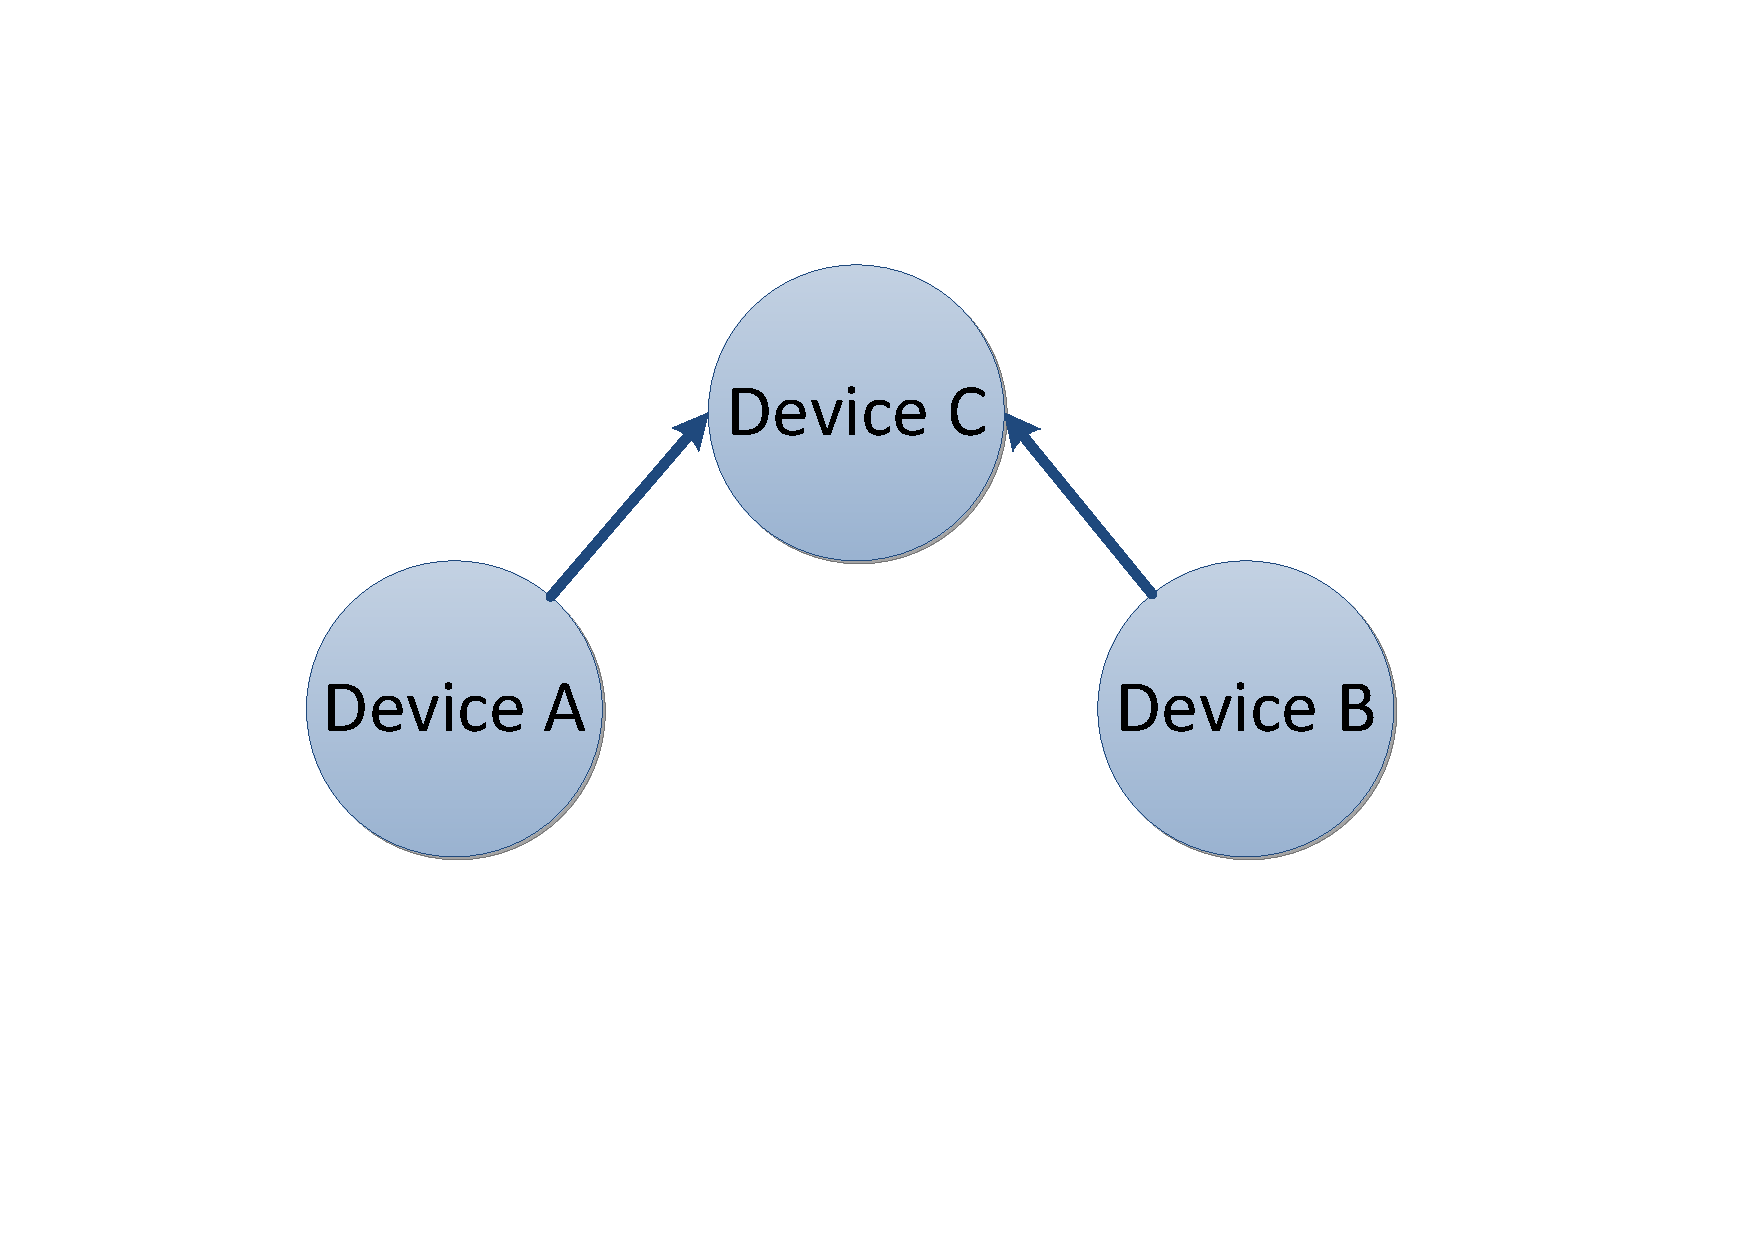
\includegraphics[width=3in]{images/relatedWork/HiddenNode.pdf}
		%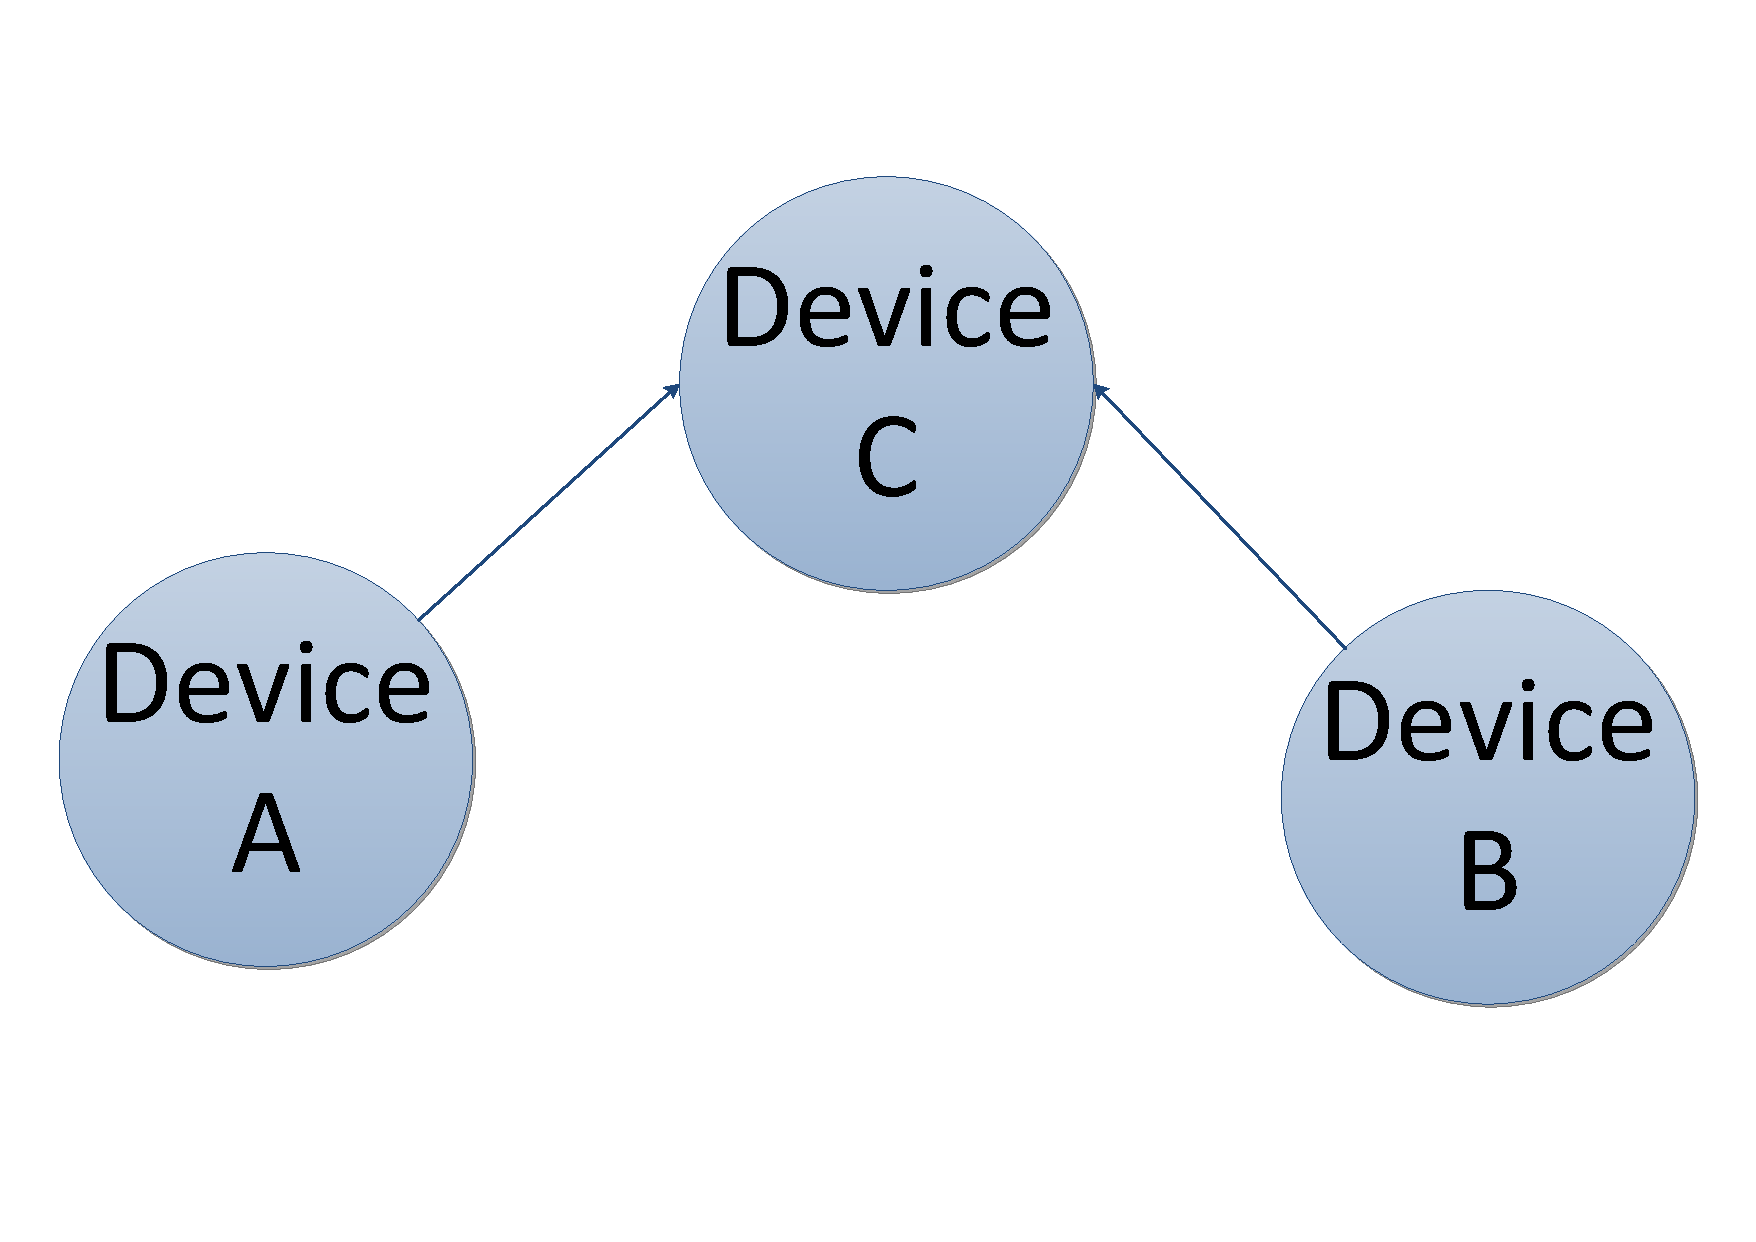
\includegraphics[width=3in]{images/relatedWork/TDMAScheduleAndHiddenNode.pdf}
	\caption{Device A and device B can both communicate with device C, but A and B are out of range of each other.}
	\label{fig:images_relatedWork_hiddenNodeProblem}
\end{figure}


\section{MAC Layer Protocols}

% What is a mac-layer protocol 
Carrier sense multiple access (CSMA)~\cite{generalCSMA, generalCSMAPart2} is a general protocol that is general to networking 
devices that have a shared channel. 
Designed by Kleinrock and Tobagi in 1975 for transmitting data over radio, CSMA requires devices to listen on the channel
to ensure no other devices are transmitting before beginning a transmission. The `carrier sense' part of the name comes from 
the device that is ready to send checking (or sensing) to see if there is already a transmission in progress. 
Since the protocol is designed to have many devices sharing the same channel, it is a 
`multiple access' protocol. CSMA has a problem called `the hidden node problem'. This arises when two 
devices that are out of radio range of each other are communicating with the same device that is in 
between the two. This problem can be seen in Figure~\ref{fig:images_relatedWork_hiddenNodeProblem}, where device A and B 
are both trying to communicate with device C. Device A and B do channel checks and do not hear any noise on the channel,
so they begin transmitting. Device C gets both transmissions at the same time, causing a collision in the messages, and 
neither of the messages are received.



%\begin{figure}[htbp]
\begin{figure}[htb]
	\centering
		
\includegraphics[width=2.5in]{images/relatedWork/CSMA.pdf}
	\caption{A CSMA handshake between two devices.}
	\label{fig:images_relatedWork_CSMA}
\end{figure}

CSMA has been adapted to WSNs by Woo and Culler~\cite{CSMA}, adding some enhancements to make 
transmissions more reliable. Woo and Culler added the idea of a two-way handshake to transmit 
messages across the network. The device sends a `ready to send' (RTS) message 
to the intended recipient (which is heard by all surrounding devices due to the shared medium). If the intended
recipient is not currently busy, it sends back a `clear to send' (CTS) message. CSMA handshaking is illustrated in  
Figure~\ref{fig:images_relatedWork_CSMA}. Woo and Culler also show that in WSNs that are largely collision-free, the ACK
step of the handshake can be dropped for energy savings. CSMA remains a major part of most WSN communication
due to its simplicity and effectiveness in detecting collisions.



\begin{figure}[bth]
	\centering
		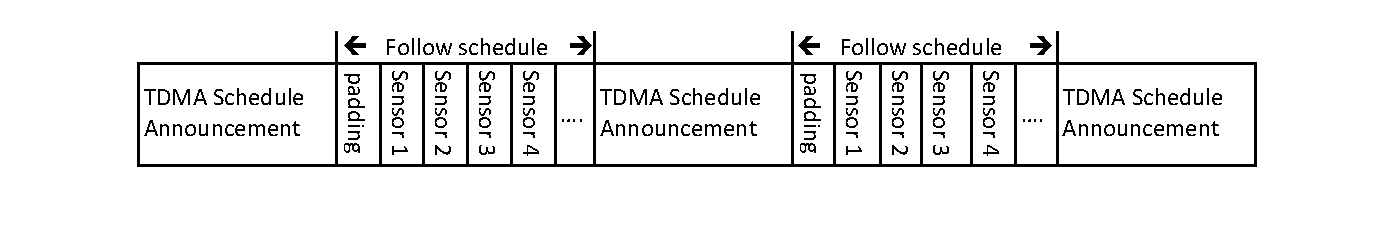
\includegraphics[width=5.5in]{images/relatedWork/tdmaSchedule.pdf}
	\caption{A sample of a TDMA schedule}
	\label{fig:images_relatedWork_tdmaSchedulev003}
\end{figure}

Time division multiple access (TDMA)~\cite{TDMA} is another method for allowing multiple 
devices to share a radio channel. Since the channel is shared, only one device can successfully
transmit at a time. If more than one device is transmitting at the same time, the messages
will collide, and neither message will be received correctly. To avoid having two devices
transmitting at the same time, a coordinator device announces a schedule that defines when and how long
the devices in the immediate area are allowed to transmit.
A visual representation of TDMA can be seen in Figure~\ref{fig:images_relatedWork_tdmaSchedulev003}.


%\section{Proactive and Reactive Networks}
%\textbf{Be nice to talk about this} Leach is reactive, teen? is reactive (like a fire alarm)


\section{Non-clustering Protocols}

Sparse Topology and Energy Management (STEM), designed by Schurgers et al.~\cite{stem} is a simple MAC protocol that uses peer to peer messaging without a clusterhead to 
send messages across a network. 
Since having the radio on drains the battery quickly, all motes cycle between listening and sleeping to conserve energy. The motes do not synchronize 
the schedule for sleeping and listening times, so motes poll neighbouring motes to send messages 
across the network. Polling wastes transmissions, since a mote will continue to send messages to a mote that is asleep until the 
mote wakes up and responds to the polling. No synchronization means that energy is wasted sending 
messages that are not received by anything.

% Directed Diffusion 
Created by Intanagonwiwat et al.~\cite{directedDiffusion, nextCentury}, Directed Diffusion 
uses peer-to-peer communication to transmit messages across the network. Directed Diffusion 
does not use clusterheads or coordinator devices to collect or route information. Since 
there are no clusterheads, all the devices in the network are tasked with 
tracking where the sink is in the network, and then transmit messages to devices in the direction
that the sink is. Intanagonwiwat et al.\ use a type of beaconing as a simple routing protocol. The
sink announces its position periodically to its neighbouring nodes. The neighbouring nodes then announce
to their neighbours that they are one hop away from the sink. This pattern continues until the entire network
knows how many hops away from the sink they are.  Directed Diffusion provides effective routing 
information with low overhead. Intanagonwiwat et al.\  considered sending some extra information with the beacons,
such as which sinks are interested in what information being sensed, but did not consider sending 
extra information about the motes along with the beacon.

% Gossiping
Gossiping is a simple way of 
increasing the chances that a message will be received at the sink. Hedetniemi et al.~\cite{gossiping} discussed
the simplicity and simple gains achieved by using gossiping in their survey paper on gossiping.
Gossiping, in general, is sending the same message along multiple routes 
to the sink. In a network with packet loss, sending multiple copies of the same message will increase the odds 
the message will be received at the sink. This also has the side-effect of possibly having the same message received at the 
sink multiple times. Another negative side-effect is that more transmissions, and therefore more power is needed to 
send one message to the sink. Though an effective way of sending messages, the cost involved in sending the messages
must be considered before using a gossiping technique.

% flooding
To quickly disseminate data, flooding~\cite{wsnSurvey} can be employed to broadcast a message across an entire WSN.
Flooding can be considered the extreme case of gossiping, where a message is announced to all surrounding 
devices, which in turn announce the same message. This is a good method for sharing routing information
quickly, but is expensive. All the devices in the network must be on, and will receive and transmit the message.
Flooding also tends to cause many collisions in the network, as all the devices will repeat the message shortly after 
receiving the message.


% smac ~\cite{smac}
S-MAC~\cite{smac} is a reliable way of moving data across a WSN without using clusterheads.
Ye et\. al outline the important features of a successful MAC layer protocol: energy efficiency, 
fairness (all motes have an equal chance of messages reaching the sink), low message latency and high throughput. 
Due to the constrained nature of WSNs, it is difficult or impossible to have all of these features, though 
networks can be tuned to enhance the desired features the network should have. An example of this 
is that a network could have better throughput, but lowered energy efficiency. S-MAC does sleep
cycling to improve the lifespan of the network, with periodic listening states to check
if any devices are trying to send to it. To avoid polling, S-MAC uses synchronization 
techniques to wake all the devices at approximately the same time, so no devices will be polling 
a device that is sleeping.




% Pegasis
Power Efficient Gathering in Sensor Information Systems (PEGASIS), designed by Lindsey and Raghavendra~\cite{pegasis},
uses global knowledge of the network to create
paths to the sink. PEGASIS saves energy by using greedy algorithms 
to create a near-optimal path to the sink. Motes hop
messages to neighbours that are closer to the sink. When a mote
receives a message, it performs message fusion on the message, then sends
the fused messages to a neighbour that is closer to the sink. Motes
using PEGASIS accept many messages and send one message per round due to this data fusion and 
hopping setup. Reducing the number of messages sent reduces the amount of energy used 
while the network runs.
PEGASIS' use of global knowledge is unrealistic in most network deployments (e.g. WSN nodes launched from a plane,
thrown into a bush) and therefore limited in its real-world applications.


\section{Clustering Protocols and Communication}

The standard approach for clustering, designed by Heinzelman et 
al.~\cite{leach}, is Low-Energy Adaptive Clustering Hierarchy (LEACH). LEACH 
is a commonly used algorithm for clustering and low energy communication. Most 
other clustering algorithms are in some way extensions of LEACH.  
Being the earliest clustering protocol for WSNs, LEACH uses somewhat 
simplistic methods for electing clusterheads. This simplicity is actually the key strength 
of LEACH, since the clusterhead election makes no assumptions about the 
network.  Heinzelman et al.\ did not consider heterogeneity or mote 
capabilities for LEACH.

Some protocols focus on sensing and reporting anomalies. Anomalies sensed
could be fires, earthquakes, security alerts, etc. Threshold sensitive Energy Efficient 
sensor Network (TEEN)~\cite{teen}, developed by Manjeshar and Agrawal, focuses on 
only reporting anomalies that are worth reporting, not wasting transmissions
on data that is not of interest. Since staying on and transmitting messages uses 
the most energy in WSNs, TEEN only sends messages if the sensor readings are
important enough to send. TEEN uses a threshold to define whether or not a
sensor reading is valuable and worth sending to the sink or not.
TEEN is a reactive-style WSN, it is not designed to regularly send information to the
sink, only if an anomaly that is being monitored occurs will a 
message be sent to the sink. This is useful for monitoring for fires or 
intruders and the like, but not useful for monitoring a resource over time.


Soro and Heinzelman~\cite{coveragepreservation} reported that, when only using 
residual energy in a mote for electing a clusterhead, the lifespan of the 
network is negatively affected when compared to using more than one factor. 
This demonstrated that the benefits of using hybrid criteria when choosing a 
clusterhead outweigh the overhead it generates. While Soro and Heinzelman showed that 
comparing more than one factor between motes in an election generates 
excessive overhead, they did not consider summarizing multiple factors into 
one hybrid criteria.

SPIN, designed by Kulik et al.~\cite{spin} uses an advertisement phase
where a mote informs surrounding motes about the message that it has. The surrounding
motes then can request the message from the mote that sent the advertisement. 
There is metadata in the advertisement that has some details about the message
that can be requested. This advertisement phase is interesting in that
any metadata could be in the advertisement message, such as information
about the mote, or messages to surrounding motes. Kulik et al.\ only considered 
sending information about the message that is ready to be sent.

Building on the foundation of LEACH, Younis and Fahmy~\cite{heed}  created 
Hybrid Energy-Efficient Distributed clustering (HEED) to address the issue of 
selecting better clusterheads. HEED uses a hierarchy much like LEACH, but uses 
more intelligence to choose the next clusterhead.  HEED uses residual power 
and a secondary parameter to create a single value describing how  well suited 
the mote is to being a clusterhead. HEED has addressed selecting better 
clusterheads based on certain parameters, but only in homogeneous networks.

Dong and Liu~\cite{resilient} created a model that chooses clusterheads based 
not only on a mote's capacity to be a clusterhead, but on data it has 
collected while the network has been alive.  If a mote had previously been 
chosen as a clusterhead, but did not do well, that mote goes to a blacklist 
and will only be chosen again if there are no known candidates to 
be a clusterhead. This use of historical data allows the network to improve 
its clusterheads over time, creating a network of clusterheads that are known 
to work well. Though Dong and Liu used knowledge of motes in the network to 
improve network lifespan, they did not consider heterogeneous networks where 
motes may have special features, such as solar panels, that could restore a 
mote with dead batteries to a useful state.

%\section{Things I'll probably delete}
%Brzozowski et al.~\cite{datareplication} investigated creating a long-term 
%data storage in long-lived WSNs.  They used data replication to ensure that 
%data is not lost during long periods when the sink is unavailable. 
%  However, Brzozowski et al.\ did not look at using heterogeneous networks 
%where some motes may have, for example, larger flash storage.
  

\section{Heterogeneous Wireless Sensor Networks}

Ou et al.~\cite{powerawareoverlay}  extended the lifespan of a heterogeneous 
WSN by making the network power-aware. Motes with larger power supplies were 
assigned the task of a clusterhead, since a clusterhead  requires more energy.  
These clusterheads were distributed around the network to create a spanning 
tree.  The power supply variance was the only heterogeneous aspect of the 
experiment and clusterheads were selected manually when the network was 
deployed, not dynamically by election.

Recognizing the lack of election protocols for heterogeneous WSN,  Smaragdakis 
et al.~\cite{stableElection} created an election protocol for heterogeneous 
WSNs.  Extending LEACH, the protocol included remaining power levels as a 
weight in clusterhead elections and concluded that this weight increased 
network lifespan.  The protocol did not  consider any other heterogeneity than 
the residual power supply. 

Brzozowski et al.~\cite{completelydistributed} explored how messages should be 
stored in heterogeneous networks, with residual energy levels being the main 
focus of the heterogeneity in the network.
Brzozowski et al.\ used a novel Media Access Control  (MAC)  protocol that 
controlled where the messages were stored and how they were routed around dying 
motes.Though Brzozowski et al. looked at routing around dead motes, they did not
consider using heterogenous motes to  extend the network lifespan even further. 
Methods such as always choosing where data should be routed, or which 
motes should be clusterheads before devices start to have critically low 
energy levels.


Hu et al.~\cite{longlivedhybrid} used two different types of motes to create a 
long-lived WSN. The motes were assigned different tasks in the network, some 
for data collection and some for routing. The authors did not consider 
self-configuring the network to utilize the heterogeneity or the possibility 
of extending the idea to more than two classes of motes. 

By creating motes with differing hardware configurations, Mhatre and 
Rosenberg~\cite{comparativestudy} showed that exploiting heterogeneity in WSNs 
can reduce network costs.  
Some of the deployed motes were inexpensive, while others were quite 
expensive. The expensive motes were configured to use the less expensive motes 
for energy-intensive tasks, allowing the more expensive motes to live longer.  
The focus was on the cost savings of a heterogeneous WSN, creating only a 
rudimentary election protocol largely based on LEACH.

Yarvis et al.~\cite{exploitHetero} described three different types of heterogeneity in 
heterogeneous WSNs, and suggested methods for best leveraging the individual 
types of heterogeneity.
The three types of heterogeneity identified were:
\begin{enumerate}
	\item \textbf{Computational Heterogeneity}. Motes have different amounts of processing power 
	available to them. Motes with more processing power should do tasks such as data fusion, or compressing messages.
	\item \textbf{Link Heterogeneity}. Some motes will have more powerful radios, providing 
	greater transmission range. Longer range allows messages to have fewer hops in the network,
	which decreases the latency time between the message being created and the message arriving 
	at its destination.
	\item \textbf{Energy Heterogeneity}. Motes have varying amounts of energy available for their use. Some motes might
	be powered externally, often called `line' or `wall' power, while other motes might have very limited
	amounts of nonrenewable battery power. Motes with more battery power should take on power-intensive tasks, 
	such as being clusterhead or performing data fusion.
\end{enumerate}
Yarvis et al.\ focused their efforts on ways of creating optimal placement of motes
with the knowledge of the heterogeneous motes in the network, and worked with S-MAC~\cite{smac} as a base
MAC protocol. They did not consider cluster-based WSNs as a way of further increasing the 
lifespan of the network.

